\chapter{Getting Started}
\label{sec:tut:started}

\us comes with a set of tools, two of which being of particular
importance:
\begin{description}
\item[\dfn{urbi}] launches an \urbi server.  There are several means
  to interact with it, which we will see later.
\item[\dfn{urbi-launch}] runs \urbi components, the UObjects, and connects
  them to an \urbi server.
\end{description}

Please, first make sure that these tools are properly installed.  If you
encounter problems, please see the frequently asked questions
(\autoref{sec:faq}), and the detailed installation instructions
(\autoref{sec:installation}).

\begin{shell}
# Make sure urbi is properly installed.
$ urbi --version
Urbi Kernel version preview/2.0/beta3-425 rev. 000913e
Copyright (C) 2005-2010 Gostai SAS.

URBI SDK Remote version preview/1.6/beta1-666 rev. 92ec3b4
Copyright (C) 2004-2010 Gostai SAS.

Libport version preview/1.0/beta1-1048 rev. f1c5170
Copyright (C) 2005-2010 Gostai SAS.
\end{shell}%$

There are several means to interact with a server spawned by \command{urbi},
see \autoref{sec:tools:urbi} for details.  First of all, you may use the
options \option{-e}/\option{--expression \var{code}} and
\option{-f}/\option{--file \var{file}} to send some \var{code} or the
contents of some \var{file} to the newly run server.  The option
\option{q}/\option{--quiet} discards the banner.

You may combine any number of these options, but beware that being
event-driven, the server does not ``know'' when a program ends.  Therefore,
batch programs should end by calling \lstinline{shutdown}.  Using a Unix
shell:

\begin{shell}[alsolanguage={[interactive]Urbi},caption={A batch session under Unix.}]
# A classical program.
$ urbi -q -e 'echo("Hello, World!");' -e 'shutdown;'
[00000004] *** Hello, World!
\end{shell}

If you are running Windows, then, since the quotation rules differ, run:

\begin{shell}[alsolanguage={[interactive]Urbi},caption={An batch session under Windows.}]
# A classical program.
$ urbi -q -e "echo(""Hello, World!"");" -e "shutdown;"
[00000004] *** Hello, World!
\end{shell}


To run an interactive session, use option
\option{-i}/\option{--interactive}.  Like most interactive interpreters,
\urbi will evaluate the given commands and print out the results.

\begin{shell}[alsolanguage={[interactive]Urbi}Unix]
$ urbi -i
[00000118] *** ********************************************************
[00000118] *** Urbi SDK version 2.0/rc-4 rev. fb573a2
[00000118] *** Copyright (C) 2005-2010 Gostai S.A.S.
[00000118] ***
[00000118] *** This program comes with ABSOLUTELY NO WARRANTY.
[00000118] *** It can be used under certain conditions.
[00000118] *** Type `license;' or `copyright;' for more information.
[00000118] ***
[00000118] *** Check our community site: http://www.urbiforge.org.
[00000118] *** ********************************************************
1+2;
[00000000] 3
shutdown;
\end{shell}%$

The output from the server is prefixed by a number surrounded by
square brackets: this is the date (in milliseconds since the server
was launched) at which that line was sent by the server. This is
useful at occasions, since \urbi is meant to run many parallel
commands.  But since these timestamps are irrelevant in most examples,
they will often be filled with zeroes through this documentation.

Under Unix, the program \command{rlwrap} provides additional services
(history of commands, advanced command line edition etc.); run \samp{rlwrap
  urbi -i}.

In either case the server can also be made available for network-based
interactions using option \option{--port \var{port}}.  Note that while
\lstinline{shutdown} asks the server to quit, \lstinline{quit} only quits
one interactive session.  In the following example (under Unix) the server
is still available for other, possibly concurrent, sessions.

\begin{shell}[alsolanguage={[interactive]Urbi},caption={An interactive session under Unix.}]
$ urbi --port 54000 &
[1] 77024
$ telnet localhost 54000
Trying 127.0.0.1...
Connected to localhost.
Escape character is '^]'.
[00000118] *** ********************************************************
[00000118] *** Urbi SDK version 2.0/rc-4 rev. fb573a2
[00000118] *** Copyright (C) 2005-2010 Gostai S.A.S.
[00000118] ***
[00000118] *** This program comes with ABSOLUTELY NO WARRANTY.
[00000118] *** It can be used under certain conditions.
[00000118] *** Type `license;' or `copyright;' for more information.
[00000118] ***
[00000118] *** Check our community site: http://www.urbiforge.org.
[00000118] *** ********************************************************
12345679*8;
[00018032] 98765432
quit;
\end{shell}%$

Under Windows, instead of using \command{telnet}, you may use
\command{urbi-console} (part of the package), which provides a Graphical
User Interface to a network-connection to an \urbi server.  To launch the
server, run:

\begin{shell}[alsolanguage={[interactive]Urbi},caption={Starting an interactive session under Windows.}]
C:\...> start urbi --port 54000
\end{shell}

and to launch the client, click on \command{urbiConsole} which is installed
by the installer.

Then, the interaction proceeds in the \command{urbiConsole} windows.
Specify the host name and port to use (\samp{127.0.0.1:54000}) in the text
field in the top of the window and click on the right to start the connection.

\begin{center}
  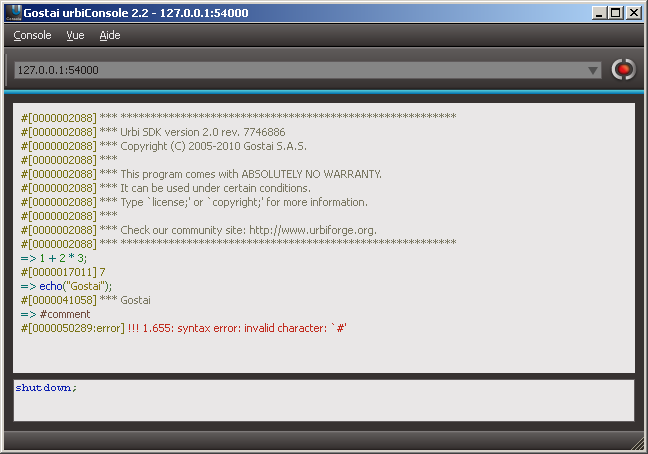
\includegraphics[width=.8\linewidth]{img/urbi-console}
\end{center}

The program \command{urbi-send} (see \autoref{sec:tools:urbi-send}) provides
a nice interface to send batches of instructions (and/or files) to a running
server.

\begin{shell}[alsolanguage={[interactive]Urbi}]
$ urbi-send -P 54000 -e "1+2*3;" -Q
[00018032] 7
# Have the server shutdown;
$ urbi-send -P 54000 -e "shutdown;"
\end{shell}

\medskip

You can now send commands to your \urbi server. If at any point you get
lost, or want a fresh start, you can simply close and reopen your connection
to the server to get a clean environment.  In some cases, particularly if
you made global changes in the environment, it is simpler to start anew:
shut your current server down, and spawn a new one.

\medskip

You are now ready to proceed to the \us tutorial: see \autoref{part:tut}.

Enjoy!

%%% Local Variables:
%%% mode: latex
%%% TeX-master: "../urbi-sdk"
%%% ispell-dictionary: "american"
%%% ispell-personal-dictionary: "../urbi.dict"
%%% fill-column: 76
%%% End:
